\documentclass[preprint,12pt]{elsarticle}

% SoftwareX manuscript
% Compile with pdflatex; bibliography is inline (thebibliography) for
% portability.

\usepackage{amsmath,amssymb}
\usepackage{graphicx}
\usepackage{booktabs}
\usepackage{url}
\usepackage{listings}
\usepackage{xcolor}

\lstset{
  basicstyle=\ttfamily\footnotesize,
  breaklines=true,
  frame=single,
  columns=fullflexible,
  backgroundcolor=\color{gray!8},
}

\journal{SoftwareX}

\begin{document}

\begin{frontmatter}

\title{fwhFoam: A Ffowcs Williams--Hawkings solver with on-surface
acoustic source localization for OpenFOAM}

\author[a]{Sparsh Sharma\corref{cor}}
\ead{sparsh.sharma@dlr.de}
\cortext[cor]{Corresponding author.}
\address[a]{German Aerospace Center (DLR), Germany}

\begin{abstract}
We present \texttt{fwhFoam}, an open-source aeroacoustic post-processing
library for the OpenFOAM computational fluid dynamics toolbox that couples
far-field noise prediction with \emph{on-surface acoustic source
localization}. Far-field sound is computed with Farassat's
formulation~1A of the Ffowcs Williams--Hawkings (FW-H) equation, evaluated
by a source-time-dominant (advanced-time) algorithm, for permeable and
impermeable integration surfaces through one unified code path and with a
uniform mean flow handled in closed form via the Garrick-triangle
emission-time relation. The distinguishing feature is a built-in
implementation of the surface sound-power density $\sigma$ derived from the
diffraction-filter theory of Delfs \& Ruck: from the same permeable-surface
data, \texttt{fwhFoam} produces a map of \emph{where on the surface the
radiated sound originates}, with an exact power identity
$\oint\sigma\,dS = P_\mathrm{far\text{-}field}$ serving as an internal
consistency check. To our knowledge no other OpenFOAM FW-H tool offers this.
The software comprises a runtime function object, an offline reprocessing
utility, a Python companion package with the localization module, and
verification suites. Far-field predictions match analytic monopole, dipole
and convected-monopole solutions to $\sim$0.1\,\% with second-order
convergence, and the $\sigma$ power identity is verified to a few tenths of
a percent on analytic sources.
\end{abstract}

\begin{keyword}
Aeroacoustics \sep Ffowcs Williams--Hawkings \sep Acoustic source
localization \sep Surface sound-power density \sep OpenFOAM \sep
Computational aeroacoustics
\end{keyword}

\end{frontmatter}

%% ------------------------------------------------------------------
\section*{Highlights}
\begin{itemize}
\itemsep0em
\item Open-source Ffowcs Williams--Hawkings acoustic solver for OpenFOAM.
\item Permeable and impermeable surfaces via one code path; closed-form mean flow.
\item Unique on-surface source localization by a surface sound-power density map.
\item A built-in identity ties the source map to the far-field radiated power.
\item Verified to $\sim$0.1\% on analytic sources with second-order convergence.
\end{itemize}

%% ------------------------------------------------------------------
\section*{Code metadata}

\begin{table}[h]
\centering
\footnotesize
\begin{tabular}{@{}p{0.42\linewidth}p{0.52\linewidth}@{}}
\toprule
\textbf{Code metadata description} & \textbf{Value} \\
\midrule
Current code version & v1.0.0 \\
Permanent link to code/repository & \url{https://github.com/Sparsh-Sharma/fwhFoam} \\
Legal code license & GPL-3.0-or-later \\
Code versioning system used & git \\
Software code languages, tools & C++ (C++14), Python 3, OpenFOAM (wmake) \\
Compilation requirements, dependencies & OpenFOAM v2306; C++14 compiler; Python$\ge$3.9 with NumPy \\
Developer documentation & \texttt{README.md}, \texttt{doc/theory.md}, \texttt{doc/fwh-data-format.md} \\
Support email for questions & sparsh.sharma@dlr.de \\
\bottomrule
\end{tabular}
\end{table}

%% ------------------------------------------------------------------
\section{Motivation and significance}
\label{sec:motivation}

Aerodynamically generated sound is a central concern in the design of
aircraft, rotors, wind turbines, ground vehicles and cooling fans. Direct
computation of the acoustic field together with the flow is prohibitively
expensive for most engineering configurations, because the acoustic
fluctuations are many orders of magnitude smaller than the hydrodynamic
ones and the far field lies many wavelengths from the source. The
established remedy is an \emph{acoustic analogy}: the near-field unsteady
flow is computed by scale-resolving CFD (LES, DES, DNS or a lattice
Boltzmann method), and an integral formulation propagates the sound to
arbitrary far-field observers at negligible additional cost.

The Ffowcs Williams--Hawkings (FW-H) equation~\cite{fwh1969} is the most
general such analogy, valid for surfaces in arbitrary motion and, in its
permeable (porous-surface) form~\cite{difrancescantonio1997,
brentner1998}, able to account for volume (quadrupole) sources by
enclosing them within an off-body integration surface. Farassat's
formulation~1A~\cite{farassat2007} is the standard time-domain
realisation and underpins most rotorcraft and turbomachinery noise
prediction tools.

Mature open-source FW-H implementations for OpenFOAM already exist; the
most established is the \texttt{libAcoustics} library~\cite{epikhin2015},
which provides Curle, Farassat~1A (permeable and impermeable) and a
wind-tunnel formulation. \texttt{fwhFoam} is not intended to replace or
compete with such tools on the far-field prediction alone, and we make no
claim of novelty for the FW-H formulation itself, which is standard. Its
contribution is twofold. First, it makes a compact, independently
verifiable FW-H capability from our institution openly available to the
OpenFOAM community, with a bundled analytic verification and convergence
suite that any user can reproduce. Second, and distinctively, it couples
the far-field prediction with \emph{on-surface acoustic source
localization}: the same permeable-surface data used for the FW-H integral
are processed into a surface sound-power density $\sigma(\mathbf{x})$ that
identifies which parts of the surface radiate to the far field. This
quantity, and the diffraction-filter theory it derives
from~\cite{delfs2024}, addresses a question the far-field signal cannot
answer --- localization of the true acoustic sources on a surface --- and
is, to our knowledge, not available in any existing OpenFOAM FW-H tool. A
built-in power identity, $\oint\sigma\,dS = P_\mathrm{far\text{-}field}$,
ties the two together and provides an internal consistency check.

%% ------------------------------------------------------------------
\section{Software description}
\label{sec:description}

\subsection{Architecture}

\texttt{fwhFoam} is organised around a mesh-independent formulation engine
that is shared by two front-ends:

\begin{itemize}
\item \texttt{libfwhFoam} --- a shared library providing the class
  \texttt{fwhFormulation1A} (the numerics) and a runtime OpenFOAM
  \emph{function object} \texttt{fwh} that samples surface data during a
  simulation;
\item \texttt{fwhSolve} --- a stand-alone utility that recomputes observer
  signals from stored surface data, allowing observers, ambient
  conditions or the mean-flow speed to be changed without re-running the
  CFD;
\item \texttt{pyfwh} --- a Python package for reading and writing the
  surface-data format, generating analytic reference fields and
  integration surfaces, computing spectra, and --- through its
  \texttt{localization} module --- evaluating the surface sound-power
  density $\sigma$;
\item \texttt{sigma\_localize} --- a driver that turns permeable
  surface-data files into a $\sigma$ map (VTK/CSV) and reports the power
  identity.
\end{itemize}

The formulation engine operates purely on raw face-centre data (position,
unit normal, area, and per-time-step samples of gauge pressure, density
and fluid velocity), so identical numerics serve the patch-based
(impermeable) and sampled-surface (permeable) paths and the runtime and
offline front-ends.

\subsection{Governing equations}

The acoustic pressure is split into thickness ($T$) and loading ($L$)
contributions. For a static integration surface $S$ with outward unit
normal $\hat{n}$ in a uniform mean flow of Mach vector
$\mathbf{M}=-\mathbf{U}_0/c_0$,
\begin{align}
4\pi p'_T(\mathbf{x},t) &= \int_S \!\Big[
  \frac{\rho_0\,\dot{U}_n}{r(1-M_r)^2}
  + \frac{\rho_0 U_n\, c_0(M_r-M^2)}{r^2(1-M_r)^3}\Big]_{\mathrm{ret}} dS,
\label{eq:pT}\\
4\pi p'_L(\mathbf{x},t) &= \int_S \!\Big[
  \frac{\dot{L}_r}{c_0 r(1-M_r)^2}
  + \frac{L_r-L_M}{r^2(1-M_r)^2}
  + \frac{L_r\,c_0(M_r-M^2)}{r^2(1-M_r)^3}\Big]_{\mathrm{ret}} dS,
\label{eq:pL}
\end{align}
with the permeable-surface source vectors
\begin{equation}
U_i = v_i + \tfrac{\rho}{\rho_0}(u_i-v_i),\qquad
L_i = p'\,\hat{n}_i + \rho\, u_i (u_n-v_n),
\label{eq:sources}
\end{equation}
where $u$ is the fluid velocity, $v$ the surface velocity, $r$ and
$\hat{r}$ the source-to-observer distance and unit vector,
$M_r=\mathbf{M}\cdot\hat{r}$, $L_M=\mathbf{L}\cdot\mathbf{M}$, subscript
$n$ a projection on $\hat{n}$, subscript $r$ on $\hat{r}$, and a dot a
source-time derivative. For a solid wall $u_n=v_n$ and
Eqs.~\eqref{eq:sources} reduce to the classical impermeable form, so no
separate code path is required.

\subsection{Advanced-time algorithm}

Rather than solving the implicit retarded-time equation, \texttt{fwhFoam}
marches in source time: an element emitting at time $\tau$ is received at
$t=\tau+T$, where the emission-to-reception delay $T$ follows from the
closed-form Garrick-triangle relation
\begin{equation}
(c_0^2-U_0^2)\,T^2 + 2(\mathbf{d}\cdot\mathbf{U}_0)\,T - |\mathbf{d}|^2 = 0,
\qquad \mathbf{d}=\mathbf{x}_{\mathrm{obs}}-\mathbf{y},
\label{eq:garrick}
\end{equation}
requiring only $|\mathbf{U}_0|<c_0$. Each element's contribution is
deposited onto a uniform observer-time grid by exact piecewise-linear
resampling between consecutive (Doppler-shifted) arrival times; time
derivatives use second-order central differences over three buffered
source levels. The scheme is single-pass and streaming (three source
levels in memory) and parallelises by having each MPI rank integrate its
own faces, the partial observer signals being combined by a fixed-size
reduction.

\subsection{On-surface source localization}

The distinguishing capability operates on the permeable-surface Cauchy
data --- the surface pressure $p$ and normal velocity $v_n=\mathbf{u}\cdot
\hat{n}$ that the FW-H surface already samples. Working per angular
frequency $\omega=c_0k$ with the complex spectra
$\phi=\hat{p}$ and $\psi=\partial\hat{p}/\partial n=-i\omega\rho_0\hat{v}_n$,
the radiating field has far-field directivity
$F(\hat{\mathbf{x}})=\frac{1}{4\pi}\oint[\,ik(\hat{\mathbf{x}}\cdot\hat{n})
\phi-\psi\,]e^{ik\hat{\mathbf{x}}\cdot\boldsymbol{\xi}}\,dS$ and radiated
power $P=\frac{1}{2\rho_0 c_0}\oint|F|^2\,d\Omega$. Carrying out the
angular integration in closed form yields an exact surface sound-power
density
\begin{equation}
\sigma(\boldsymbol{\xi}) = \frac{1}{32\pi^2\rho_0 c_0}\,\mathrm{Re}\!\oint
\Big[ k^2 (\hat{n}\!\cdot\!\mathbf{W}\!\cdot\!\hat{n}')\,\phi\phi'^{*}
- ik(\hat{n}\!\cdot\!\mathbf{V})\phi\psi'^{*}
+ ik(\hat{n}'\!\cdot\!\mathbf{V})\psi\phi'^{*}
+ J_0\,\psi\psi'^{*} \Big]dS(\boldsymbol{\xi}'),
\label{eq:sigma}
\end{equation}
with closed-form kernels $W_{ij}=4\pi[\delta_{ij}j_1(z)/z-\hat{d}_i\hat{d}_j
j_2(z)]$, $V_i=4\pi i\,j_1(z)\hat{d}_i$, $J_0=4\pi j_0(z)$, where
$\mathbf{d}=\boldsymbol{\xi}-\boldsymbol{\xi}'$, $z=k|\mathbf{d}|$,
$\hat{d}=\mathbf{d}/|\mathbf{d}|$. By construction $\oint\sigma\,dS=P$, so
the localization map and the far-field power are two views of the same
data and must agree. On a rigid wall ($\psi=0$) only the pressure block
survives, recovering the classical rigid-surface density~\cite{delfs2024}.
The density is signed, reflecting that radiated power is a two-point
quantity.

\subsection{Usage}

The runtime function object is enabled from \texttt{system/controlDict};
switching between an impermeable and a permeable surface is a change of a
single sub-dictionary:

\begin{lstlisting}
fwh1
{
    type    fwh;   libs (fwhFoam);
    c0      340.29;   rho0 1.225;   U0 (0 0 0);
    surface { type patches; patches (cylinder); }   // impermeable
    observers { mic1 { position (0 10 0); } }
    executeControl timeStep;  executeInterval 8;
}
\end{lstlisting}

%% ------------------------------------------------------------------
\section{Illustrative examples}
\label{sec:examples}

\subsection{Analytic verification}

The distributed test suite feeds exact acoustic fields onto a geodesic
icosphere enclosing the sources and compares the predicted observer
pressure with the analytic far field. Because the surface data are exact,
a correct formulation must reproduce the analytic signal to discretisation
accuracy. Table~\ref{tab:analytic} lists the relative $L_2$ error for
three canonical cases, isolating the thickness term (monopole), the
loading term (dipole) and the convective/Garrick terms (convected
monopole at Mach~0.3). All radiating directions agree to within about
0.1\,\%.

\begin{table}[h]
\centering
\caption{Relative $L_2$ error of \texttt{fwhFoam} against analytic
far-field solutions (icosphere surface, subdivision level~3, 1280 faces,
64 samples per period).}
\label{tab:analytic}
\begin{tabular}{@{}lll@{}}
\toprule
Case & Term exercised & Relative $L_2$ error \\
\midrule
Monopole (medium at rest)   & thickness $\dot U_n$          & $1.6\times10^{-3}$ \\
Dipole (medium at rest)     & loading $L_r,\dot L_r$        & $7\times10^{-4}$--$1.6\times10^{-3}$ \\
Convected monopole, $M=0.3$ & Garrick delay + $(M_r-M^2)$   & $1.6\times10^{-3}$ \\
\bottomrule
\end{tabular}
\end{table}

\subsection{Convergence}

Figure~\ref{fig:convergence} shows the error of the monopole case as the
surface resolution and the time step are refined. Both sequences exhibit
second-order convergence (observed orders $p\approx2.6$ in space and
$q\approx2.3$ in time), consistent with midpoint-rule surface quadrature
and central-difference time derivatives applied to a smooth field.

\begin{figure}[h]
\centering
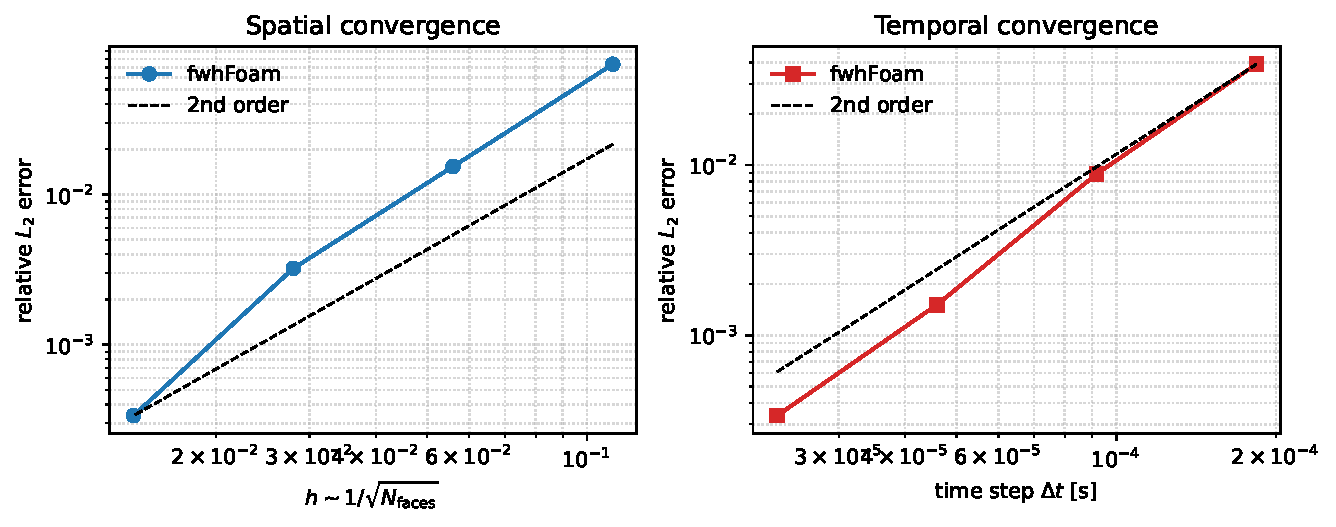
\includegraphics[width=0.9\linewidth]{figs/convergence.pdf}
\caption{Spatial (left) and temporal (right) convergence of the relative
$L_2$ error for the analytic monopole. Dashed lines indicate second-order
slopes.}
\label{fig:convergence}
\end{figure}

\subsection{Verification of the source-localization density}

The power identity underlying $\sigma$ is verified independently of the
FW-H solver. Exact monopole and dipole fields are placed on a geodesic
icosphere enclosing the source, and three quantities are compared: the
analytic radiated power (from the surface acoustic intensity of the exact
field), the far-field power from the directivity $F$, and the integral
$\oint\sigma\,dS$ of the two-point density~\eqref{eq:sigma}. For 1280 faces
they agree to $2.9\times10^{-3}$ (relative), and $\sigma$ reproduces the
correct spatial structure: uniform over the sphere for the isotropic
monopole, and vanishing at the poles while peaking at the equator for the
dipole --- the $\cos^2$ radiation pattern. This confirms both the magnitude
and the localization content of the density.

\subsection{Aeolian tone of a circular cylinder}

The tutorial \texttt{cylinderAeolianTone} computes laminar flow past a 2D
circular cylinder at $Re=100$ with the incompressible \texttt{pimpleFoam}
solver and applies the runtime \texttt{fwh} function object to the
cylinder wall (impermeable surface). Vortex shedding produces a
fluctuating lift and hence a dipole tone at the Strouhal frequency.
Figure~\ref{fig:cylinder} shows the predicted far-field pressure spectrum,
whose fundamental coincides with the shedding frequency inferred from the
lift coefficient, and the characteristic dipole directivity that peaks
normal to the mean flow.

\begin{figure}[h]
\centering
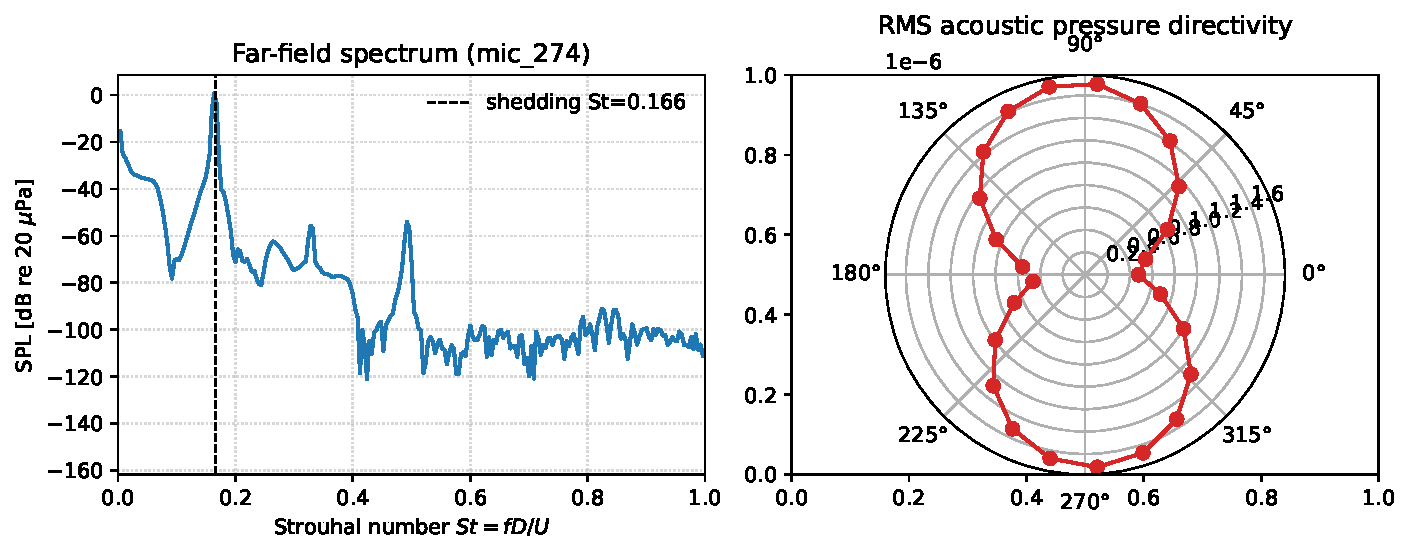
\includegraphics[width=0.9\linewidth]{figs/cylinder.pdf}
\caption{Aeolian tone of a cylinder at $Re=100$: (left) far-field pressure
spectrum at the cross-flow observer, showing the tone at the shedding
Strouhal number; (right) root-mean-square acoustic pressure directivity,
exhibiting the lift-dipole lobe pattern.}
\label{fig:cylinder}
\end{figure}

The same simulation, sampled on a permeable cylindrical control surface of
radius $8D$, yields the source-localization density~\eqref{eq:sigma} at the
shedding tone (Fig.~\ref{fig:sigma}). The density is concentrated on the
downstream sector of the control surface, where the unsteady wake crosses
it, and forms a signed lobe pair --- reflecting that radiated power is a
two-point rather than a pointwise quantity. Its surface integral reproduces
the independently evaluated far-field power to machine precision, the
built-in identity confirming the internal consistency of the computation on
genuine CFD data. The map thus attributes the tonal radiation to a
localized region of the surface rather than to the surface as a whole.

\begin{figure}[h]
\centering
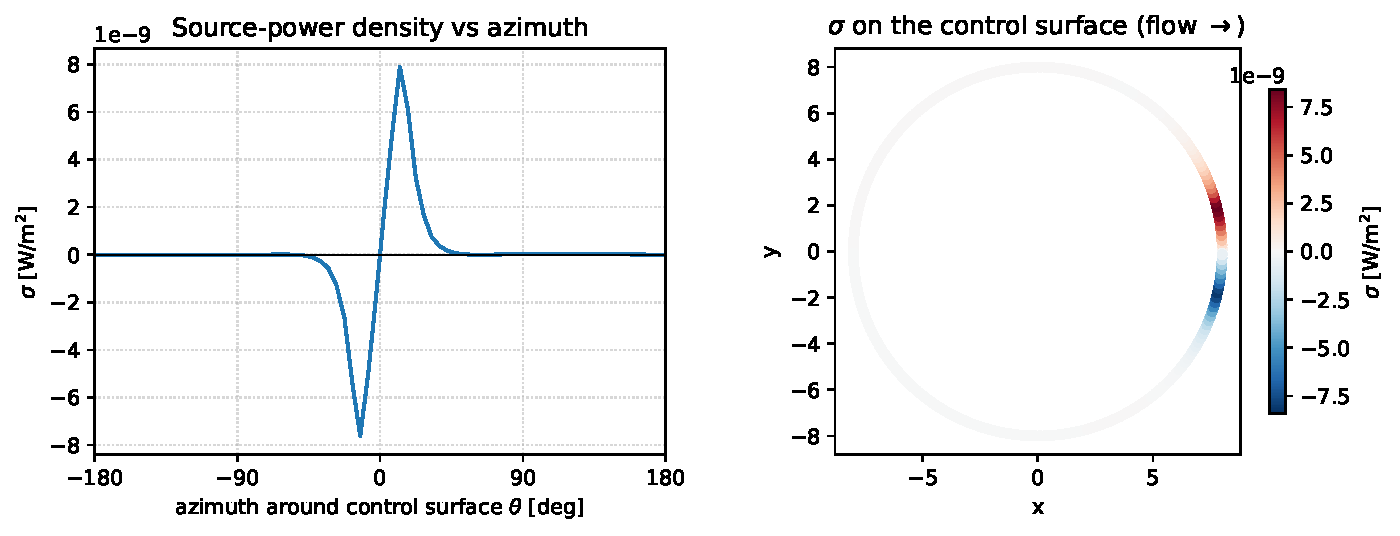
\includegraphics[width=0.9\linewidth]{figs/sigma_cylinder.pdf}
\caption{Source-power density $\sigma$ on the permeable control surface
($r=8D$) at the shedding tone: (left) azimuthal profile around the surface;
(right) $\sigma$ over the surface (mean flow left to right). The density
localizes to the downstream wake-crossing sector and is signed, integrating
to the far-field radiated power $\oint\sigma\,dS = P$ to machine precision.}
\label{fig:sigma}
\end{figure}

%% ------------------------------------------------------------------
\section{Impact}
\label{sec:impact}

\texttt{fwhFoam} contributes to the OpenFOAM aeroacoustics ecosystem in two
ways. As a far-field solver it provides a compact, documented and
independently verified FW-H capability that complements existing
libraries; the offline \texttt{fwhSolve} utility decouples the expensive
CFD from the inexpensive acoustic post-processing, so observer arrays,
ambient conditions and mean-flow speeds can be explored without re-running
the flow solver. Its more significant impact is to bring \emph{acoustic
source localization} into a standard CFD workflow: the surface sound-power
density $\sigma$ turns an FW-H integration surface, normally used only to
obtain a far-field signal, into a diagnostic that shows which surface
regions actually radiate. This directly supports noise-reduction design ---
identifying the parts of an airframe, edge or porous treatment responsible
for the radiated sound --- which a far-field spectrum alone cannot. Because
$\sigma$ is computed from the same permeable-surface data as the FW-H
integral and carries a built-in consistency identity, it adds this
capability at negligible marginal cost and with a self-check. The bundled
analytic verification and convergence suites provide a template for
reproducible validation, and the mesh-independent formulation engine is a
foundation for moving-surface (rotating-frame) and frequency-domain
extensions.

%% ------------------------------------------------------------------
\section{Conclusions}
\label{sec:conclusions}

We have described \texttt{fwhFoam}, a compact and independently verifiable
Ffowcs Williams--Hawkings solver for OpenFOAM supporting permeable and
impermeable integration surfaces and a uniform mean flow, whose
distinguishing feature is a built-in on-surface acoustic source
localization: the surface sound-power density $\sigma$, computed from the
same data as the far-field integral, with an exact power identity as an
internal check. The far-field solver is verified against analytic
monopole, dipole and convected-monopole solutions to about 0.1\,\% with
second-order convergence, and the localization density is verified through
its power identity on analytic sources to a few tenths of a percent.
Planned extensions include moving and rotating integration surfaces, the
diffraction-filter projection for rigid-wall data, and a frequency-domain
formulation.

%% ------------------------------------------------------------------
\section*{Acknowledgements}
Computations were performed on the DLR CARA high-performance computing
cluster.

\begin{thebibliography}{9}

\bibitem{fwh1969}
J.~E. Ffowcs Williams, D.~L. Hawkings,
Sound generation by turbulence and surfaces in arbitrary motion,
Phil. Trans. R. Soc. A 264 (1151) (1969) 321--342.

\bibitem{difrancescantonio1997}
A.~Di Francescantonio,
A new boundary integral formulation for the prediction of sound radiation,
J. Sound Vib. 202 (4) (1997) 491--509.

\bibitem{brentner1998}
K.~S. Brentner, F.~Farassat,
Analytical comparison of the acoustic analogy and Kirchhoff formulation
for moving surfaces, AIAA J. 36 (8) (1998) 1379--1386.

\bibitem{farassat2007}
F.~Farassat,
Derivation of Formulations 1 and 1A of Farassat,
NASA TM-2007-214853, 2007.

\bibitem{casalino2003}
D.~Casalino,
An advanced time approach for acoustic analogy predictions,
J. Sound Vib. 261 (4) (2003) 583--612.

\bibitem{epikhin2015}
A.~Epikhin, I.~Evdokimov, M.~Kraposhin, M.~Kalugin, S.~Strijhak,
Development of a dynamic library for computational aeroacoustics
applications using the OpenFOAM open source package,
Procedia Computer Science 66 (2015) 150--157.

\bibitem{delfs2024}
J.~W. Delfs, B.~Ruck,
A quantity to identify turbulence related sound generation on surfaces,
J. Sound Vib. 586 (2024) 118490.

\end{thebibliography}

\end{document}
